\documentclass[12pt,a4paper,onecolumn]{article}
\usepackage[utf8]{inputenc}
\usepackage[ngerman]{babel}
\usepackage{datetime}
\usepackage[autostyle]{csquotes}
\usepackage{hyperref}
\usepackage{graphicx}
\usepackage[toc]{glossaries}
\usepackage{xcolor}
\setcounter{tocdepth}{5}
\setcounter{secnumdepth}{5}
\makeglossaries

\newcommand\titleofdoc{StayHealthy} % Put your document title in this argument
\newcommand\GroupName{Team 6} % Put your group name here. If you are the only member of the group, just put your name


\newglossaryentry{Trainingseinheit}
{
    name=Trainingseinheit,
    description={Is a markup language specially suited 
    for scientific documents}
}

\newglossaryentry{Trainingsplan}
{
    name=Trainingsplan,
    description={Ein Trainingsplan ist ein wöchentlicher Plan der aus verschiedenen und mindestens einer Trainingseinheit besteht.}
}

\newglossaryentry{Mahlzeit}
{
    name=Mahlzeit,
    description={Mathematics is what mathematicians do}
}

\newglossaryentry{Ernährungsplan}
{
    name=Ernährungsplan,
    description={Mathematics is what mathematicians do}
}

\newglossaryentry{Zeitplan}
{
    name=Zeitplan,
    description={Mathematics is what mathematicians do}
}

\newglossaryentry{Sportler}
{
    name=Sportler,
    description={Mathematics is what mathematicians do}
}

\newglossaryentry{Personaltrainer}
{
    name=Übung,
    description={Mathematics is what mathematicians do}
}

\begin{document}
\begin{titlepage}
   \begin{center}
        \vspace*{4cm} % Adjust spacings to ensure the title page is generally filled with text

        \Huge{\titleofdoc} 

        \vspace{0.5cm}
        \LARGE{Software Architektur Spezifikation}
            
        \vspace{3 cm}
        \Large{\GroupName}
       
        \vspace{0.25cm}
        \large{Andreas Wirth, Marco Klein, Khader AlHamed, Denis Manherz}
       
        \vspace{3 cm}
        \Large{\today}% change date format to dd.mm.yyyy
        
        \vspace{0.25 cm}
        \Large{Software Praktikum}
       

       \vfill
    \end{center}
\end{titlepage}
\setcounter{page}{2}
\tableofcontents
\newpage

\section{Dokumentinformationen} 
\subsection{Änderungsgeschichte}
\begin{center}
\begin{tabular}{ |c|c|c|c| } 
 \hline
 Datum & Version & Änderung & Autor\\ 
 \hline
 25.04.2022 & 0.0 & Inhaltsverzeichnis & Denis Manherz \\ 
 \hline
 25.04.2022 & 1.0 & Erster Entwurf & Denis Manherz \\ 


 \hline 14.05.2022 & 1.3 & UML Diagramm & Marco Klein \\ 

 \hline
\end{tabular}
\end{center}

\section{Einführung}
\subsection{Definitionen und Abkürzungen}
GUI \\
bzw. beziehungsweise

\subsection{Referenzen}
 -Unterlagen aus der Vorlesung SE von Prof. Dr. Doering\\
\subsection{Übersicht}
Dieses Dokument beschreibt die Art und den Aufbau der Softwarearchitektur von StayHealthy.
Es werden einzelne Packages und deren Schnittstellen beschrieben. Zusätzlich werden Sequenzdiagramme für die jeweiligen Use Cases geliefert. 

\section{Architektonische Darstellung}
Die Softwarearchitektur teilt sich auf in 4 Bereiche: Dateneingabe, Ausgabe, Datenhaltung und Analyse der Daten.

\section{Architektonische Ziele und Einschränkungen}
Der Arbeitsaufwand ist durch diese Aufteilung möglichst gleich auf die Teammitglieder verteilt.
Um einen raschen Arbeitsfortschritt gewährleisten zu können werden Abhängigkeiten zwischen Teilbereichen der Architektur möglichst klein gehalten. Des weiteren können die Teammitglieder mit den einzelnen Levels schon von Anfang an bis zu einer gewissen Stufe mit ihrer Arbeit beginnen. Erst bei Überschneidung müssen auf ein oder mehrere andere Teammitglieder gewartet werden. 

\section{Logische Architektur}
Die Architektur ist in die Pakete GUI und Datenverarbeitung unterteilt.\\ Die einzelnen Pakete enthalten mehrere Operationen. \\
Die GUI besteht aus der Anmeldung/ Registrierung, Abmeldung, dem Anlegen eines Profils/ einer Mahlzeit/ einer Trainingseinhreit und außerdem die Auswahl der Ansicht. 
\\
Es könnnen der Zeitplan bearbeitet sowie direkte Trainings- bzw. Ernährungspläne bearbeitet werden. 
Außerdem ist die Bearbeitung des Profils möglich. 
\subsection{Übersicht}
%hier paketdiagramm und uml-klassendiagramm ,evtl. Tabelle die Funktionalität der Klassen erklärt
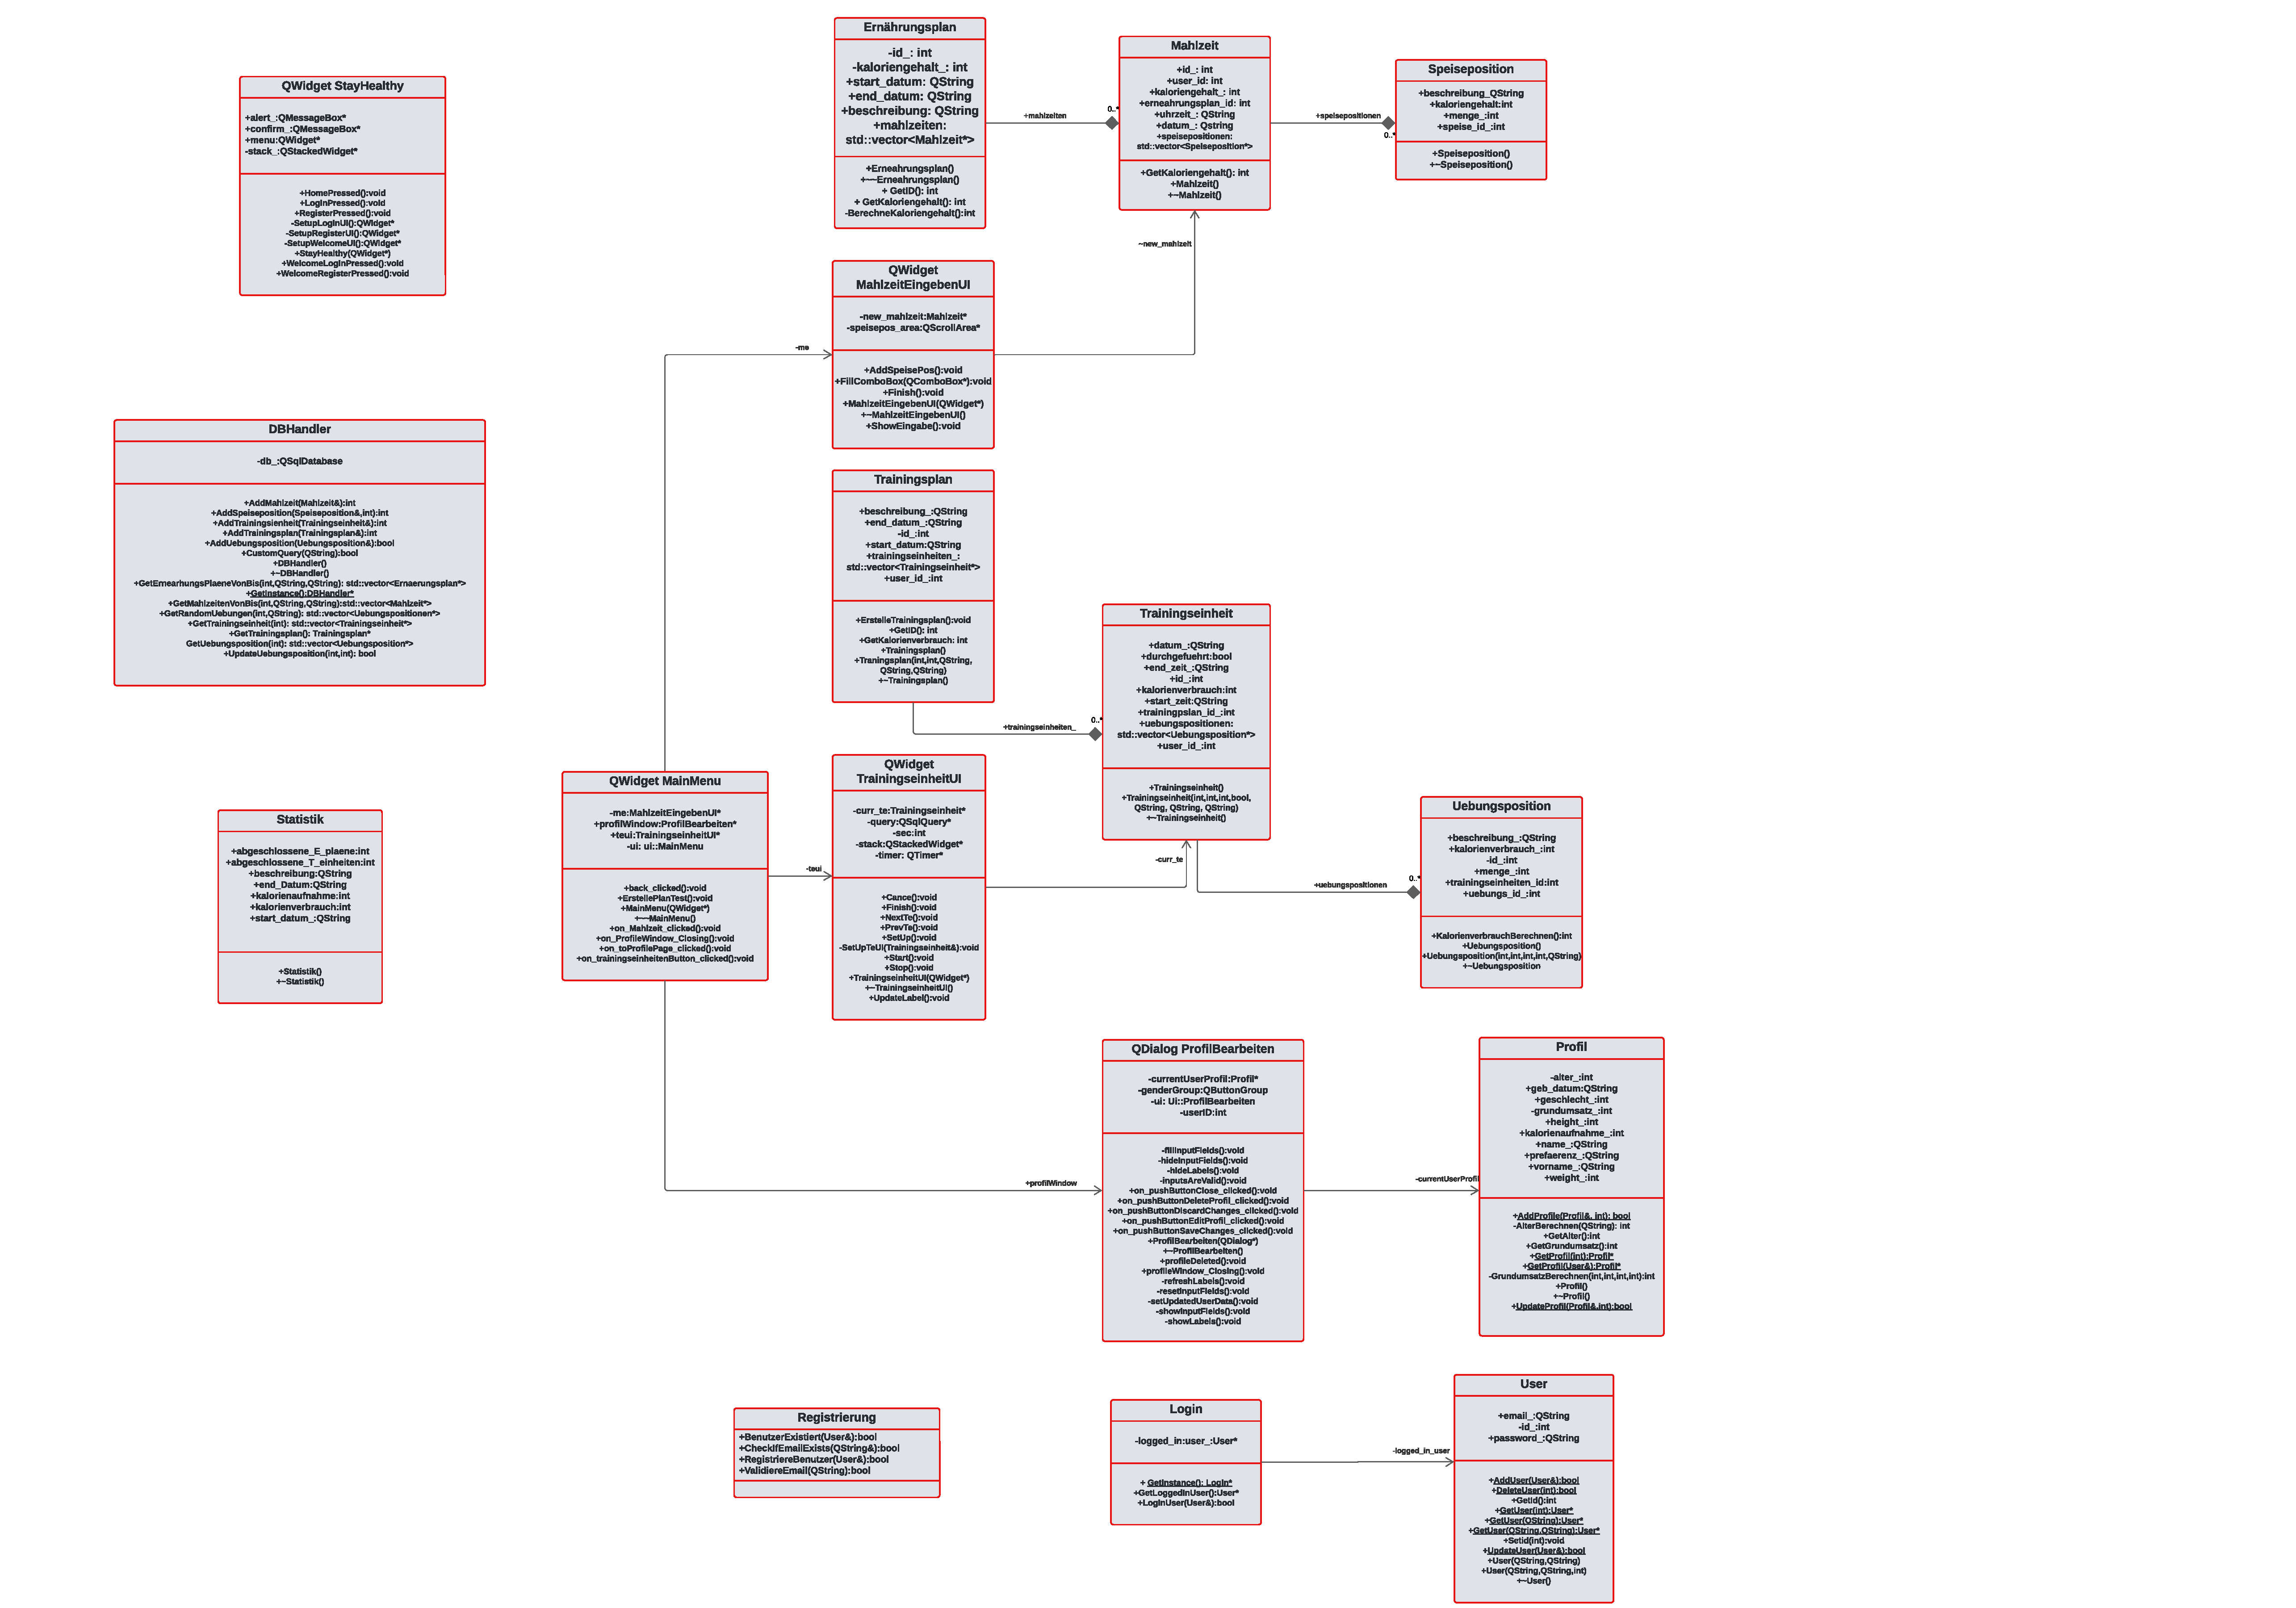
\includegraphics[scale=0.2]{StayHealthy-UML.pdf}\\
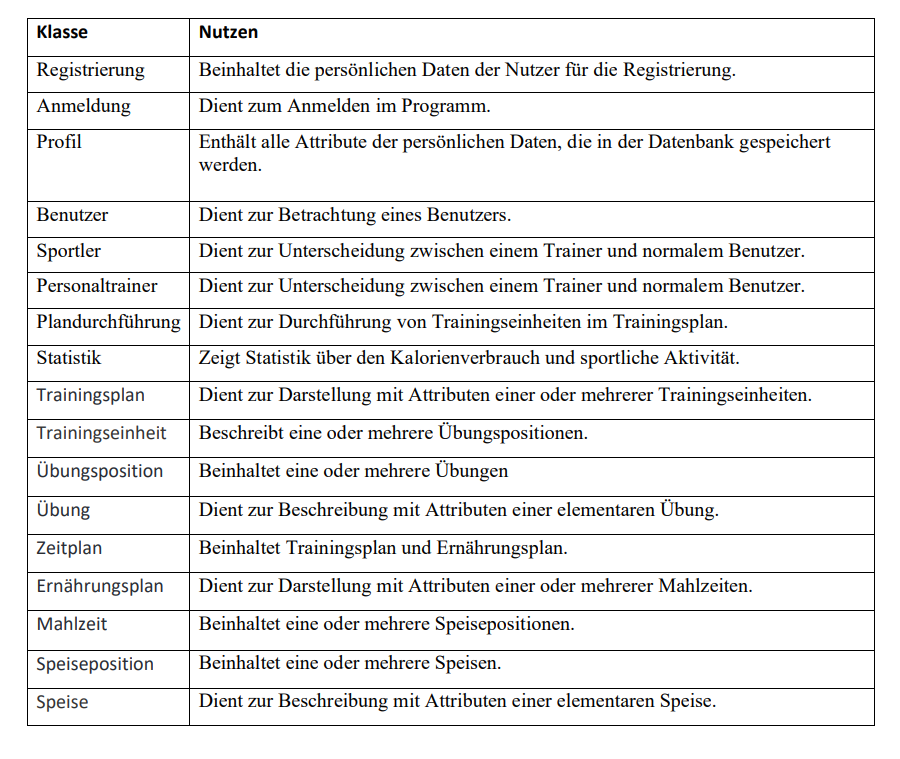
\includegraphics[scale=0.6]{Screenshot (7).png}

\subsection{Design Pakete}
\subsubsection{Package GUI}
\paragraph{Beschreibung des Package}\mbox{}\\
Die GUI bietet dem Benutzer die Möglichkeit durch die Anwendung zu navigieren und sich Ansichten anzeigen zu lassen oder Eingaben zu tätigen.
\paragraph{Diagramme}\mbox{}\\
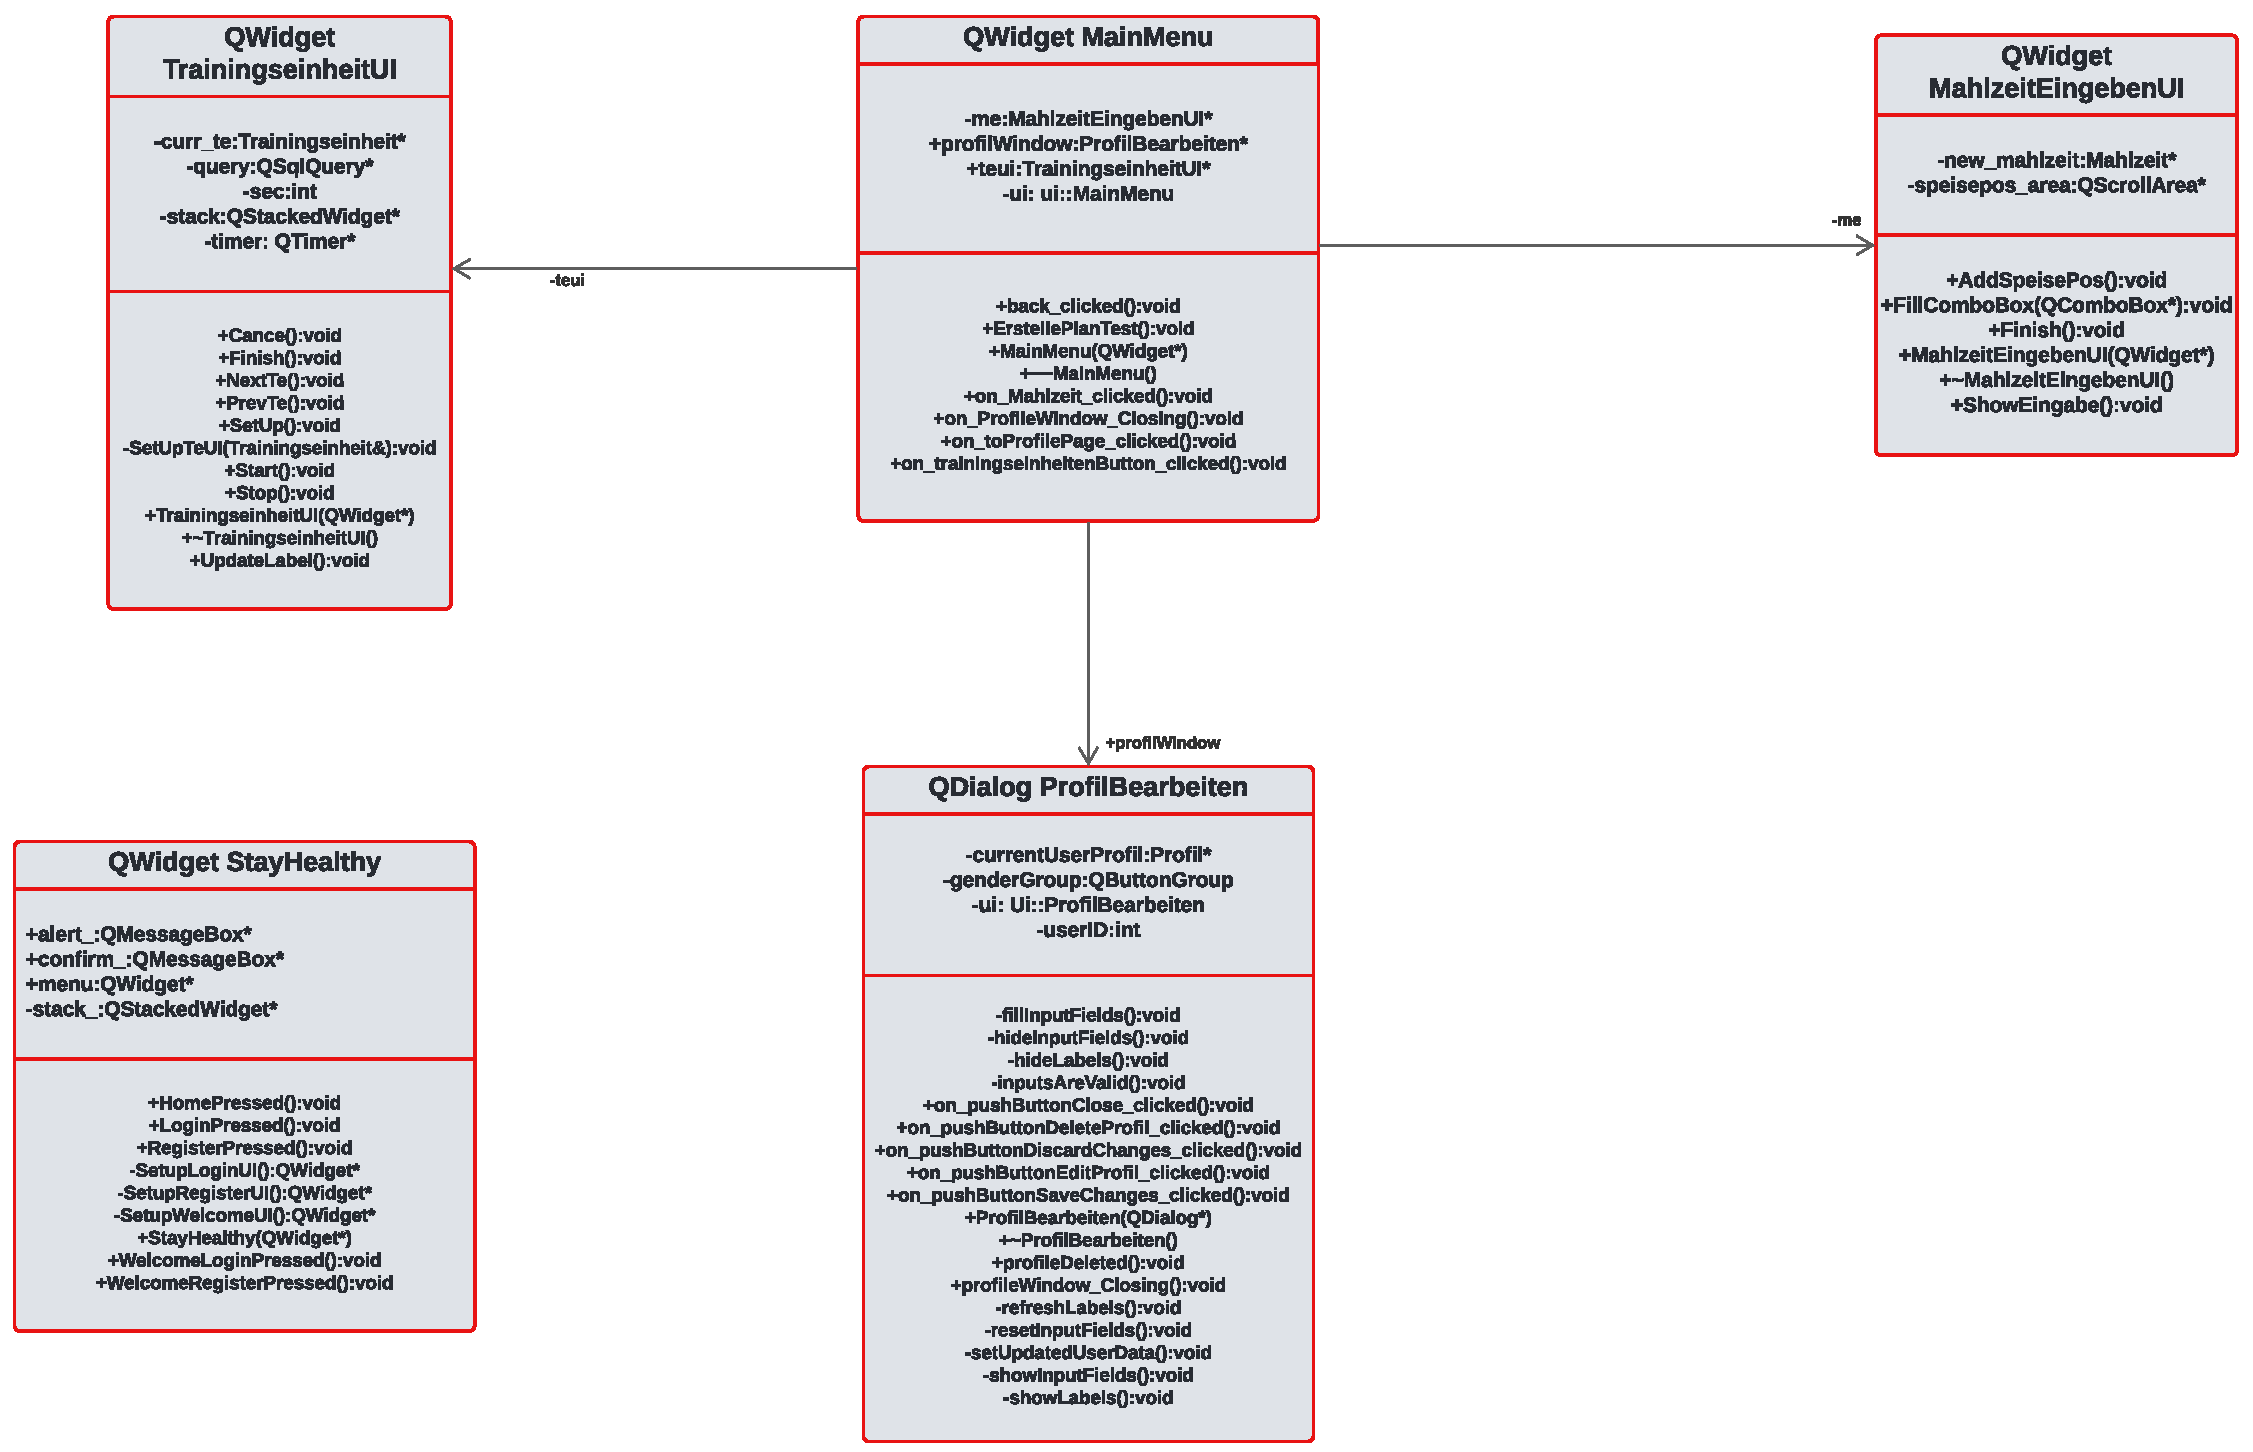
\includegraphics[scale=0.3]{StayHealthy-GUI.pdf}
\paragraph{Schnittstellen}\mbox{}\\
Datenverarbeitung
\paragraph{Operationen}\mbox{}\\
\subparagraph{Profil bearbeiten}\mbox{}\\
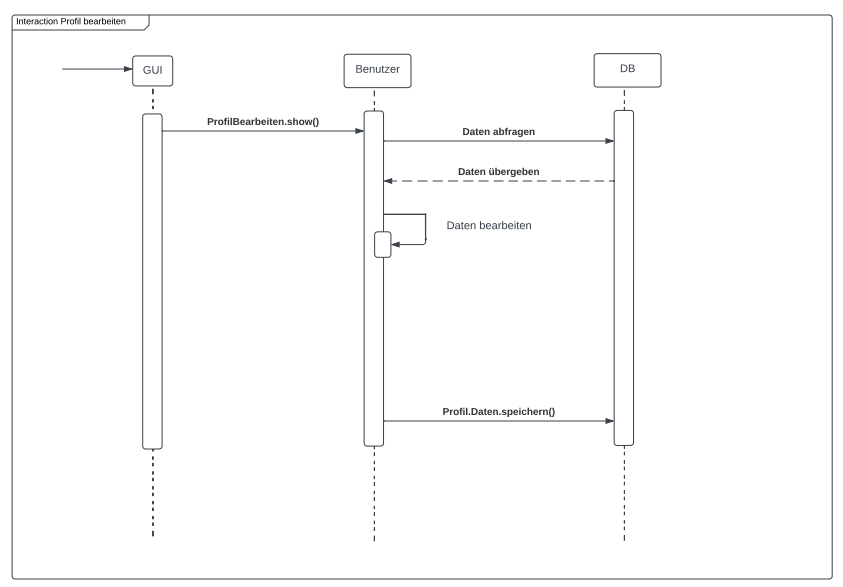
\includegraphics[scale=0.6]{Screenshot (3).png}

\subsubsection{Package Logik}
\paragraph{Beschreibung des Package}\mbox{}\\
Das Paket Logik erzeugt oder bearbeitet Objekten der Klassen Benutzer,Trainingsplan, Trainingseinheit, Übungsposition sowie Enährungsplan, Mahlzeit und Speiseposition. Diese Klassen sind als logischer Teil der Software notwendig und erleichtern den Speichervorgang sowie das Abrufen der eingepflegten Daten in der Software.
\paragraph{Diagramme}\mbox{}\\
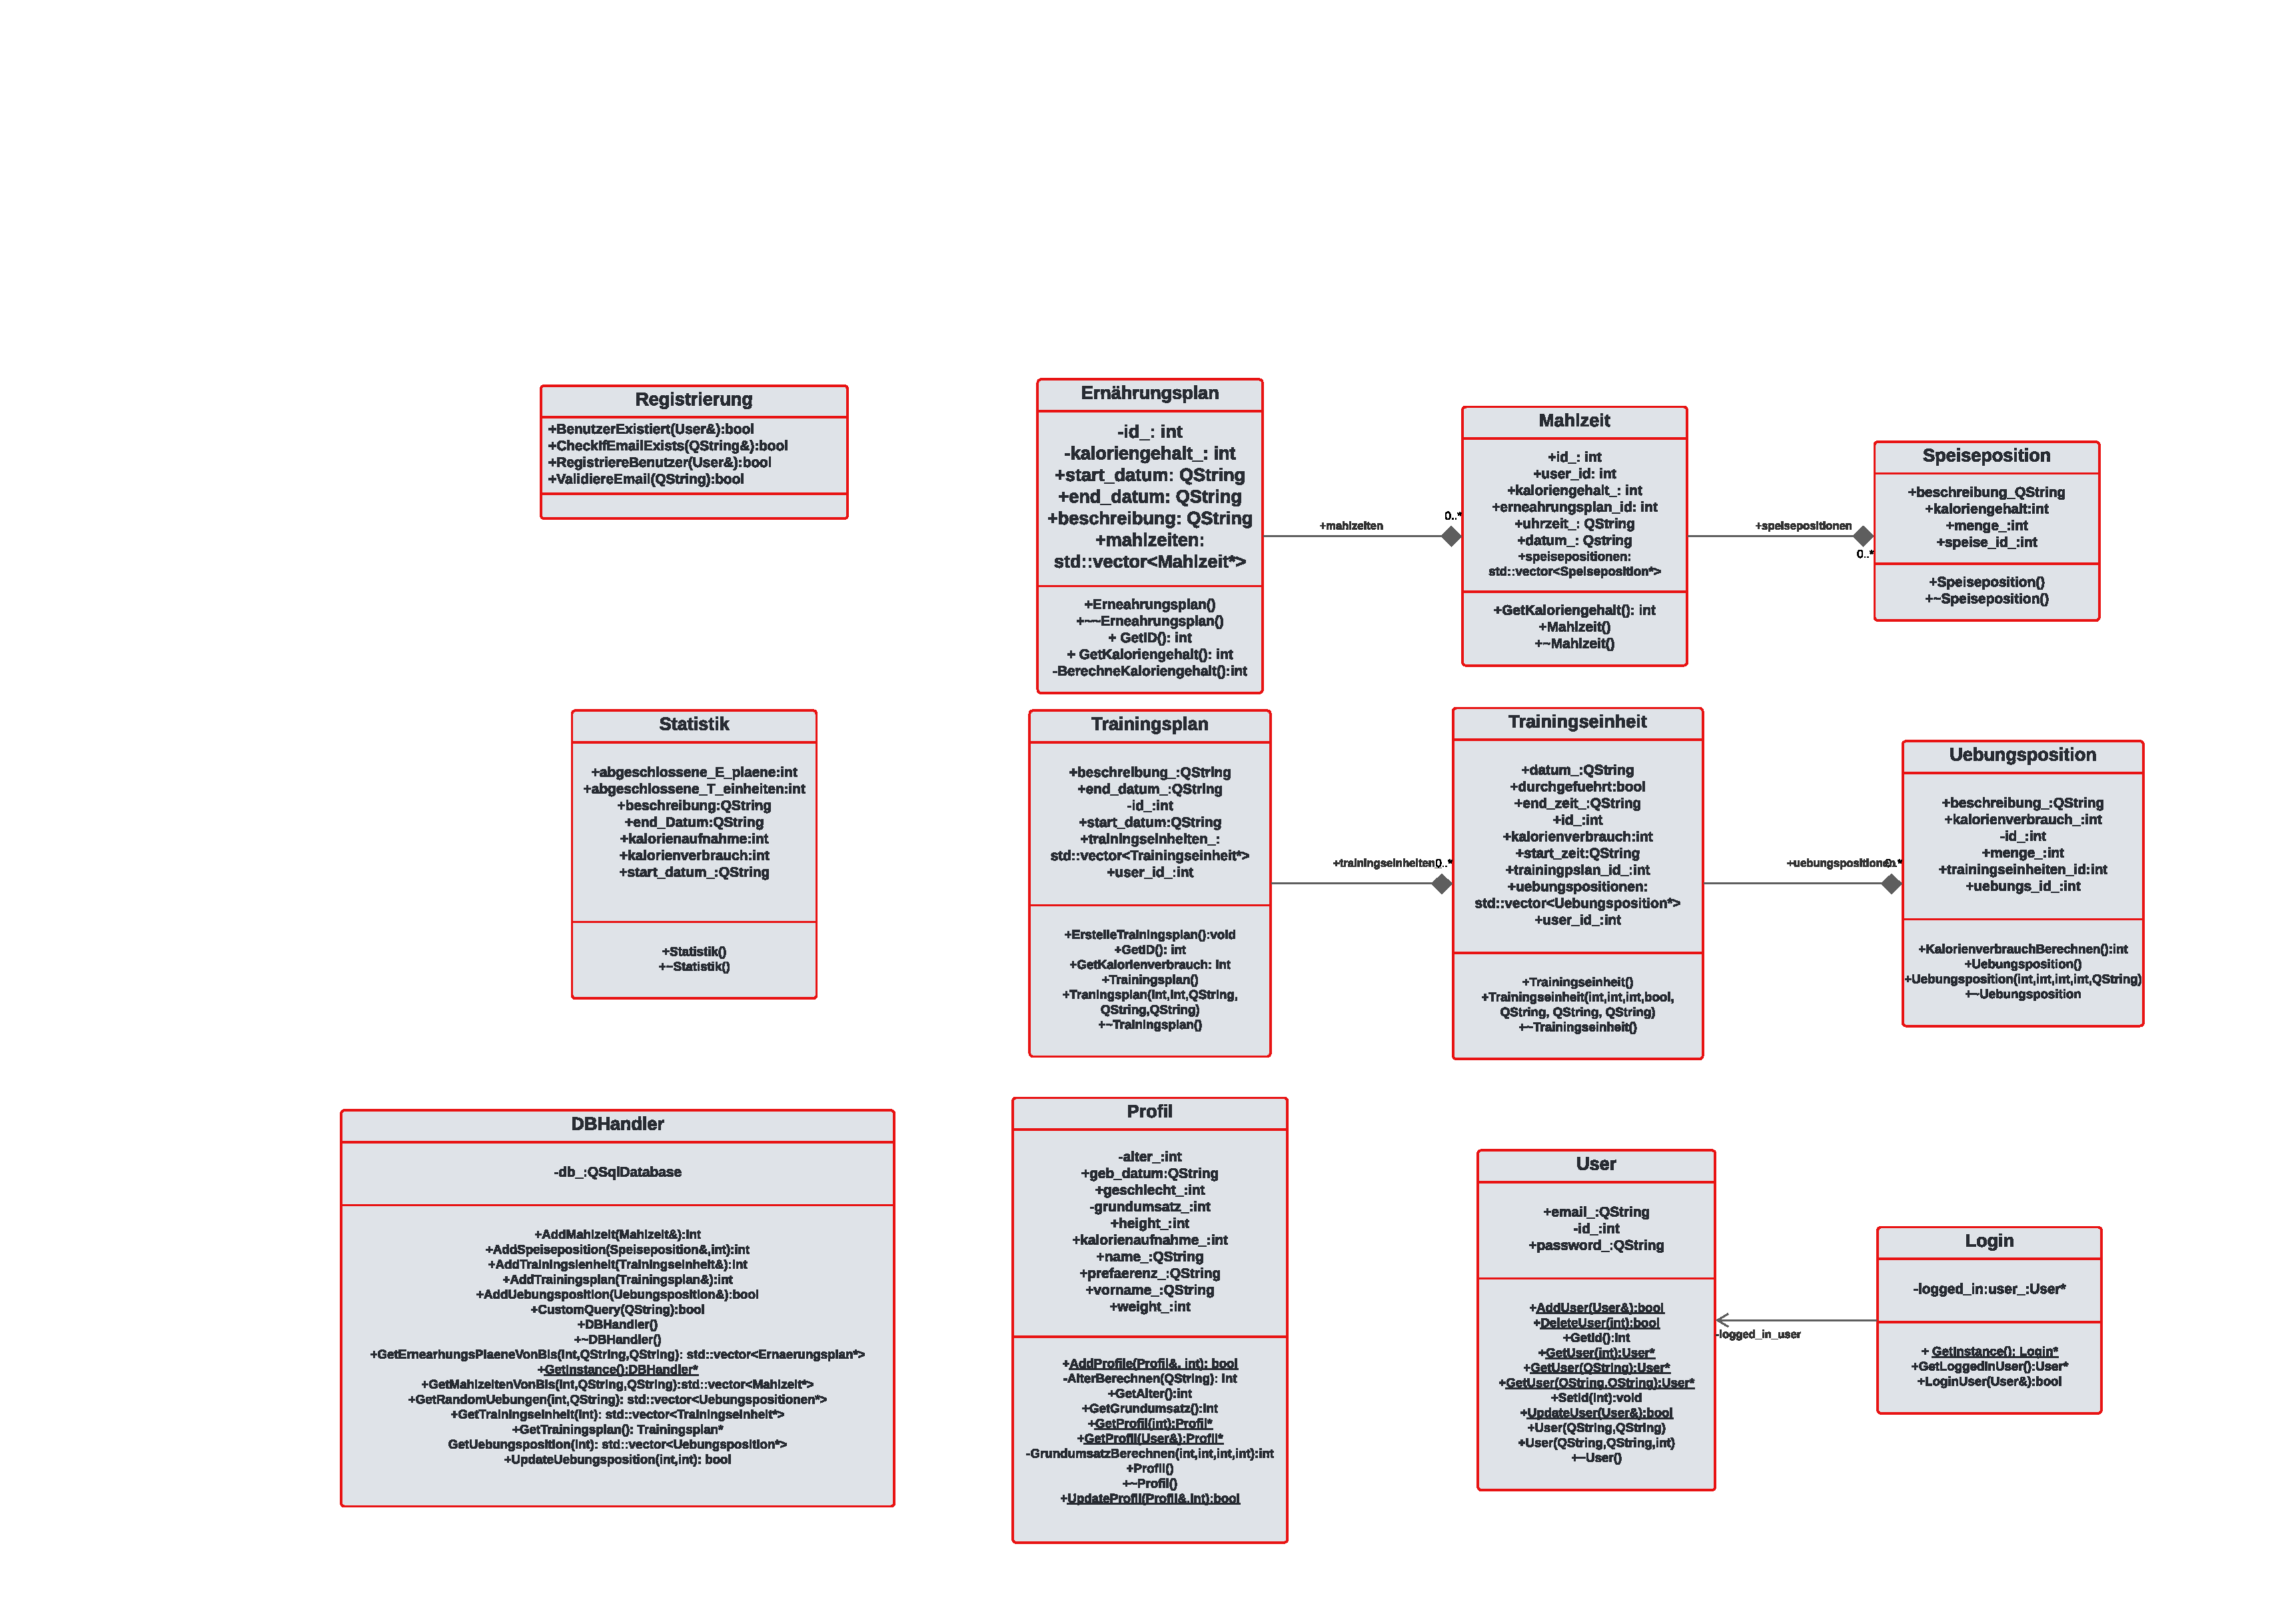
\includegraphics[scale=0.3]{StayHealthy-Logik.pdf}

\paragraph{Schnittstellen}\mbox{}\\
Das Paket Logik hat nur eine Schnittstelle zur Datenbank. Diese wird benötigt, um Daten aus der Datenbank in logische Klassen zu übersetzen.
\paragraph{Operationen}\mbox{}\\
\subparagraph{Benutzer anmelden}\mbox{}\\
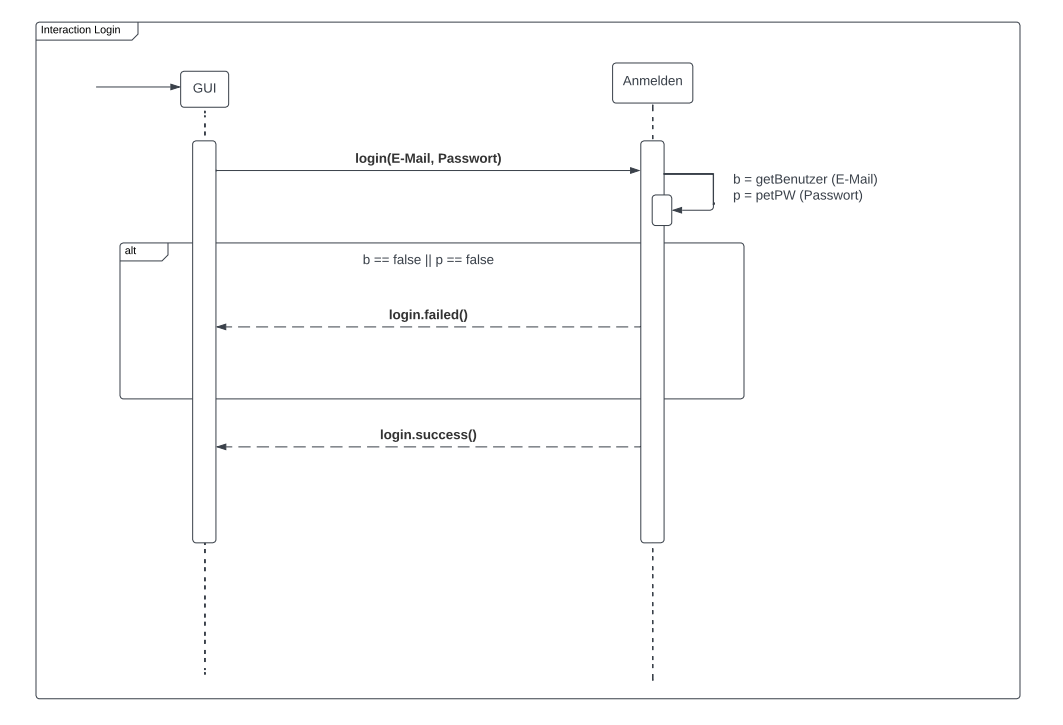
\includegraphics[scale=0.6]{Screenshot (2).png}

\section{Physikalische Sicht}
Für die Benutzung der StayHealthy Software wird lediglich ein Computer mit dem Betriebssystem MS Windows 10 oder neuer benötigt. Vorinstallierte Programme werden nicht benötigt. Auch spezielle Hardwareteile, die an den PC angeschlossen werden, werden nicht gebraucht. Der Benutzer interagiert mit der Anwendung über das GUI mit Maus und Tastatur. Internetverbindung ist benötigt um Die Daten auf den Datenbank hochzuladen.

\section{Prozesse und Threads}
Der Benutzer gibt in der GUI EMail, Passwort ein diese werden als QStrings an die Datenverarbeitung weitergeleitet, wo der Benutzer in der Datenbank registriert wird. Analog zur Registrierung kann sich der Benutzer anmelden. Nach dem anmelden hat der Benutzer zugriff auf alle Funktionalitäten der Anwendung. Er kann seine Daten ändern und sich seine Daten ansehen.
Die Daten die aus der GUI hervorgehen werden in der Datenverarbeitung verarbeitet und wenn nötig in der Datenbank hinterglegt, gelöscht, verändert oder ausgegeben.

\section{Datenspeicherung}
%hier uml datanbankdiagramm
\includegraphics[scale=0.4]{tem6.png}

\section{Größen und Leistung}
\begin{itemize}
    \item Pro Anwendungsinstanz kann sich nur ein Benutzer anmelden.
    \item Benutzer und deren Profile sind einzigartig.
    \item Benutzerdaten werden maximal 1 Jahr gespeichert.
    \item Ein Benutzer kann pro Woche einen Plan erstellen diesen aber beliebig ändern.
    \item Ein Benutzer kann pro Tag maximal 30 Mahlzeiten bzw. Trainingseinheiten speichern.
\end{itemize}

\section{Risiken}
%braucht man das hier auch ? oder beziehen sich diese risiken auf implementierungs dinge
Nachfolgend werden alle nicht trivialen Risiken des Projekts aufgeführt: \\
- Aufgrund mangelnder Kommunikation auftretende Programmierfehler, die zu Speicherlecks und Sicherheitslücken führen können\\
- Probleme auf anderen Betriebssystemen \\
- zu große Menge an Daten die in der Datenbank gespeichert werden und einen daraus resultierenden Programmabsturtz. \\
- Die Eingaben der Daten sind nur auf Deutsch verfügbar.

\section{Off-the-shelf Software}

\textbf{Bestriebssystem:} 
\begin{itemize}
    \item Windows
\end{itemize}

\textbf{Bibliotheken:} 
\begin{itemize}
    \item QtGui
    \item QtWidgets
    \item QtSql
    \item QtCore
\end{itemize}

%
%Verfahren zur Versionskontrolle eindeutig beschrieben und umgesetzt siehe checkliste ms2
%für jedes arbeitspaket ein branch wenn arbeitspaket fertig merge wenn abhängigkeiten fertig
%
%
%Daten sind sehr individuell d.h. keine 2 Trainingseinheiten die erstellt wurden passen wahrscheinlich zum gleichen %benutzer
%
%Statistik wird aus Daten von Trainingseinheiten und Mahlzeiten erstellt
%
%Auto Trainingsplan erstellen dieser besteht aus 3 einheiten (Zeiten kann man ja dann ändern) eine einheit besteht aus 5 übungen diese verbrauche (WOchenkalorienaufnahme / 3 ) kalorien. sodass am ende alle kalorien verbraucht ssind und natürlich grundumsatz miteinbeziehen 
%
%evtl können gleiche übungspositionen in mehreren Trainingseinheiten enthalten sein, da sie die richtige kalorienanzahl verbrauchen
%

\printglossary
\end{document}


